\documentclass[reprint,aps,prl,twocolumn,superscriptaddress,groupedaddress]{revtex4-2}
\usepackage[UTF8]{ctex}


\usepackage[final]{graphicx}
\usepackage[hidelinks]{hyperref}
\usepackage{bm,physics,amsmath,amssymb,xcolor}
\usepackage[normalem]{ulem}

\usepackage{centernot}
\usepackage{braket}
\usepackage{tabularx}
\usepackage{booktabs}
\usepackage{pifont}
\usepackage{colortbl}
\usepackage{amsthm}
\usepackage{soul}
\usepackage{epsfig}

\setcounter{secnumdepth}{4}
\usepackage{titlesec}

\newcommand{\eomo}{$E_1$-$M_1$}
\newcommand{\eoet}{$E_1$-$E_2$}
\newcommand{\etet}{$E_2$-$E_2$}
\newtheorem{theorem}{定理}
\newtheorem*{remark}{定理}
\definecolor{CL_Yellow}{HTML}{E69E5B}
\colorlet{LightYellow}{CL_Yellow!25}
\definecolor{CL_Pink}{HTML}{9E5BE6}
\colorlet{LightPink}{CL_Pink!25}
\definecolor{CL_Green}{HTML}{9EE65B}
\colorlet{LightBlue}{CL_Green!25}
\newcommand{\cg}[3]{C^{#1}_{#2;#3}}
\newcommand{\ii}{\mathrm{i}}

\newcommand{\correction}[2]{\textcolor{red}{\sout{#1}} \textcolor{blue}{#2}}
\newcommand{\hide}[1]{}

\usepackage{printlen}
\makeatletter
\edef\textFontName{\fontname\csname
  \f@encoding/\f@family/\f@series/\f@shape/\f@size\endcsname}
\edef\mathFontName{\fontname\textfont0}
\edef\mathLetterFontName{\fontname\textfont1}
\makeatother
\newcommand{\printsizes}{
    \uselengthunit{in}~\\
    textwidth: \printlength{\textwidth}\\
    linewidth: \printlength{\linewidth}\\
    text height: \printlength{\textheight}\\
    font name: \textFontName \\
    font size: \the\fontdimen6\font\relax
}
\begin{document}
\title{振动-转动螺旋二色性的自下而上分析}
\author{Mateja Hrast}
\email[]{mateja.hrast@ist.ac.at}
\affiliation{奥地利科学技术研究所 (ISTA), Am Campus 1, 3400 Klosterneuburg, Austria}
\author{Georgios M. Koutentakis}
\email{georgios.koutentakis@ist.ac.at}
\affiliation{奥地利科学技术研究所 (ISTA), Am Campus 1, 3400 Klosterneuburg, Austria}
\author{Mikhail Maslov}
\email{mikhail.maslov@ist.ac.at}
\affiliation{奥地利科学技术研究所 (ISTA), Am Campus 1, 3400 Klosterneuburg, Austria}
\author{Mikhail Lemeshko}
\email{mikhail.lemeshko@ist.ac.at}
\affiliation{奥地利科学技术研究所 (ISTA), Am Campus 1, 3400 Klosterneuburg, Austria}
\date{\today}
\begin{abstract}
螺旋二色性(Helical Dichroism, HD)是一种利用光的轨道角动量(Orbital Angular Momentum, OAM)解析分子手性的新兴方法。本研究突破传统理论对HD的假设,基于分子对称性与转动本征态构建了严格的HD分析理论框架。我们推导出转动选择定则,明确证明即使对于无远场OAM的光束,HD现象也仅源于光的自旋-轨道耦合作用。这些发现细化了观测HD的实验条件,不仅为已有实验结果提供理论解释,更为未来基于结构光的手性传感设计提供了重要指导。
\end{abstract}
\maketitle
许多具有生物和化学重要性的分子以手性对形式存在——这两种不可重叠的镜像版本称为对映体。分离对映体的能力对于制药和农用化学品工业至关重要\cite{MAIER2001}。这一点在甲基苯丙胺分子上体现得尤为明显:其R-对映体是有效的鼻充血缓解剂,而S-对映体则是导致成瘾流行的精神活性药物~\cite{barkholtz2023}。高度的经济相关性推动了对映选择性合成手性分子的研究,例如通过不对称催化或生物催化,或使用手性辅助剂\cite{Brown1989}。然而,这些先进合成技术需要进一步优化,并通过对映选择性过程评估对映体纯度。这个关键步骤目前仍面临技术挑战。现有化学方法各自存在局限性,包括高成本、耗时、适用性有限和可靠性不足等问题\cite{qian2023}。本文从化学物理的视角提出替代方案,旨在通过光-物质相互作用评估对映体纯度。得益于光学物理的快速发展\cite{Koch2019},这种方法为手性识别提供了经济高效且高度可控的途径。

数十年来,左旋和右旋圆偏振光吸收差异(即圆二色性CD)\cite{deutsche1970,Holzwarth1974}一直被用于手性介质的光谱分析\cite{Miles2021}。然而,圆二色性依赖于光的自旋角动量这一有限资源。与此同时,Allen等人\cite{Allen1992}的开创性研究表明,光除了携带自旋角动量外,还具有轨道角动量(OAM)。与自旋不同,光束携带的OAM量子数在理论上是无界的。携带OAM的光束具有螺旋状波前结构,这种手性特征可能与物质的手性相匹配,为对映选择性应用提供了前所未有的可能性。

这种设想最终催生了利用OAM诱导过程检测对映体纯度的具体方案,特别是螺旋二色性(HD)\cite{ANDREWS2004,Ye2019,Li2021},其被认为是对CD的重大改进\cite{Ye2019,Li2021}。Forbes和Andrews的奠基性理论研究\cite{Forbes2018,Forbes2019,Forbes2021}系统分析了光-物质相互作用多极展开项的对称性,指出电偶极-磁偶极(\eomo)、电偶极-电四极(\eoet)和电四极-电四极(\etet)项可作为手性鉴别依据。他们推导了\eoet跃迁振幅与分子多极矩的关系表达式,但未尝试用分子转动态来评估这些多极矩。实验方面,早期研究未能观测到HD信号\cite{Araoka2005,Loeffler2011},但近期实验声称实现了观测\cite{Rusak2019,Zhang2020,Rouxel2022,Begin2023,Jain2023}。不过这些实验装置极为复杂,且尽管有理论认为需要强聚焦条件\cite{Forbes2019},但迄今尚未有理论阐明观测到的二色性起源。

本研究通过揭示转动振动光谱中产生HD的条件填补了这一空白。我们首先概述基于分子多极矩的手性检测方法,推导\eoet二色性观测的对称性要求。利用新近发展的分子-光相互作用哈密顿量\cite{Maslov2024,Maslov_Thesis},我们推导出\eoet项诱导的转动振动跃迁选择定则。分析表明,傍轴拉盖尔-高斯(LG)光束无法产生真正的HD(即源于OAM转移的HD)。特别地,强聚焦条件至关重要——因为光的自旋-轨道耦合(SOC)\cite{Bliokh2015}能使OAM转移至手性分子,从而产生傍轴近似下不存在的HD贡献。我们进一步证明,即使不携带远场OAM的高斯光束,在强聚焦条件下也能产生HD信号。这些发现完善了转动振动光谱中HD的理论基础,为未来利用结构光进行对映体选择性实验和技术设计提供了指导。

现有多种对映体敏感方法基于分子多极矩分析。标准手性检测方法——(振动)圆二色性涉及\eomo项,已有详尽研究\cite{Stephens1985,BUCKINGHAM1987,Mun2019,Lovesey2019}。其原理在于:手性分子的电偶极矩在镜像反射下会改变符号(矢量特性),而磁偶极矩(赝矢量)则保持不变。两种多极共存表明分子缺乏镜面对称(严格说是非真转轴),从而定义其手性。该方法要求分子对称性至少允许一个非零偶极矩,因此可检测多种对称群的手性分子。但\eomo项产生的二色性仅取决于场强,这使得其他可通过场结构增强二色性的机制更具吸引力。

例如,相位敏感微波三波混频技术\cite{Patterson2013,Patterson2013PRL}利用偶极矩乘积$d_xd_yd_z\neq 0$作为手性判据\cite{Patterson2013,Ordonez2018,Ayuso2022}。对称性分析表明,只有完全不对称($C_1$)手性分子符合此条件。

我们探索了另一条路径——源于分子电偶极矩和电四极矩的手性条件。\eoet项诱导的二色性可通过适当结构的光场增强,这使其成为未来对映体敏感技术的理想候选。最近,磁偶极-磁四极($M_1$-$M_2$)耦合也被提出作为HD来源,其对称性与\eoet项等效\cite{Ji2024}。但由于多极展开中高阶项(如\etet)的跃迁概率极低,实验检测极具挑战性。
本文剩余部分将重点研究源自\eoet 项的二向色性特征。基于简单的点电荷模型,我们推导出以下条件(证明详见补充材料\footnote{参见补充材料,其中包含参考文献\cite{Maslov2024,Maslov_Thesis,Lax1975,Bliokh2015,Bliokh2023}}):\\
\textit{若在主轴坐标系中,对于不同的$\mu, \nu, \rho \in \{x,y,z\}$坐标,偶极矩与四极矩的乘积$d_{\mu}Q_{\nu \rho} \neq 0$,则该分子具有手性。}\\
该条件以往总是与螺旋二向色性(HD)相关联\cite{ANDREWS2004,Forbes2018}。然而,本研究表明:即使光场未向分子内部自由度传递轨道角动量(OAM),该条件同样能产生鉴别效应。本文中HD特指伴随OAM转移的二向色性效应,而不涉及OAM转移的效应(即便使用携带OAM的光束)则称为圆二向色性(CD)。

表~\ref{tab:chiral_multipole_dofs}总结了\eoet 项可诱导二向色性的手性点群。在纯转动光谱中,仅需考虑分子的永久多极矩;而振动-转动光谱中,振动跃迁可能改变分子态对称性,因此需结合终态振动能级不可约表示$V$的变换特性进行分析,这使得更多手性群可被检测。该表列出了各手性点群中呈现二向色性的$V$表示。
\begin{table}[ht!]
    \centering
    \caption{所有可能手性点群的旋转光谱与旋转振动光谱中的\eoet ~手性特征。对于旋转振动光谱,我们给出了与非零手性特征相关联的振动模式不可约表示。}
     \setlength\tabcolsep{3pt}
\begin{tabular}{p{70pt} | c c c c c c c c c c}
\toprule
     Point group     & $C_1$ & $C_2$ & $C_{n\geq 3}$ & $D_2$ & $D_{n\geq 3}$ & $T$ & $O$ & $I$ \\ \midrule
     Rotational      & \textcolor{black}{\ding{52}} & \textcolor{black}{\ding{52}}& \textcolor{red}{\ding{56}}  & \textcolor{red}{\ding{56}}  & \textcolor{red}{\ding{56}}  & \textcolor{red}{\ding{56}}  & \textcolor{red}{\ding{56}}  & \textcolor{red}{\ding{56}} \\
     Ro-vibrational  & $A$ & $A$, $B$ & $E_1$ & $B_{1, 2, 3}$ & $E_1$ & $T$ & \textcolor{red}{\ding{56}} & \textcolor{red}{\ding{56}} \\
     \bottomrule
\end{tabular}
     \label{tab:chiral_multipole_dofs}
 \end{table}
如表\ref{tab:chiral_multipole_dofs}所示,\eoet项仅能通过保持分子对称性的跃迁(纯转动及平凡表示$A$的振动-转动)识别$C_1$和$C_2$对称性的手性分子。鉴于大多数已知手性分子(即不对称陀螺分子\cite{Bernath})具有$C_1$对称性,本文研究范围限定于此。

不对称陀螺转子哈密顿量的本征态在转动基$\ket{J,M,K}$\cite{Bernath}中表示为:
\begin{equation}
    \ket{J_{N_p,N_o}(M)}=\sum_KC_K\ket{J,M,K}.
    \label{basisChange}
\end{equation}
其中$J$为总角动量量子数,$M$和$K$分别为${\bm J}$在实验室量子化轴和本体固定主轴上的投影。非对称陀螺指标$N_p$与$N_o$是纯扁长/扁圆解中$K$的极限值,并非好量子数。由于量子数$J$和$M$不受基变换\eqref{basisChange}影响,我们进一步推导转动基$| J, M, K \rangle$内电偶极($E_1$)与电四极($E_2$)跃迁的选择定则。

初始$i=\ket{J,M,K}$到终态$f=\ket{J,M',K'}$的分子转动态跃迁速率可通过文献\cite{Maslov2024,Maslov_Thesis}中的光-物质相互作用哈密顿量计算,其跃迁振幅为:
\begin{equation}
    \mathcal{M}_{i\to f}=\sum_{lm\mu}\mathcal{I}^{\text{vib}; l,\mu}\,\mathcal{I}^{\text{CM}; l,m}\,\mathcal{I}^{\text{rot}; l,m,\mu,\sigma}_{J,M,K,J,M',K'}\,,
    \label{eq_transition_matrix}
\end{equation}
式中$l=0$和$l=1$分别对应偶极与四极跃迁,$m = 0, \pm 1, \dots, \pm l$表示传递给分子的OAM,$\mu = 0, \pm 1, \dots, \pm (l+1)$覆盖球基下所选多极矩的所有分量,$\sigma =0, \pm 1$为光的偏振分量。振动项$\mathcal{I}^{\text{vib}; l,\mu}$与质心项$\mathcal{I}^{\text{CM}; l,m}$分别参数化分子与光场特性。本文重点关注支配角动量选择定则的转动跃迁振幅$\mathcal{I}^{\text{rot};l,m,\mu,\sigma}_{J,M,K,J,M',K'}$,其总结于表~\ref{SelectionRules}。
\begin{table}[ht!]
    \centering
    \begin{tabular}{c c}\hline
    \toprule
        \textbf{$E_1$ transition} & \textbf{$E_2$ transition}  \\
        \midrule
        $\Delta J\leq 1$ &  $\Delta J\leq 2$ \\
        $\Delta M=-\sigma$ & $\Delta M=m-\sigma$ \\
        $\Delta K=\pm\mu$ & $\Delta K=\pm\mu$ \\
        $J=0\not\to J'=0$ &  (see \cite{Note1}\\
        $\ket{J,0,K}\not\to\ket{J,0,K'}$ &  for details)\\
    \bottomrule
\hline
    \end{tabular}
    \caption{电偶极子 ($E_1$) 与四极子 ($E_2$) 跃迁在转动态 $\ket{J,M,K}$ 之间的选择定则。关于禁戒跃迁的详细信息请参阅 \cite{Note1}。}
    \label{SelectionRules}
\end{table}
可以证明$\mathcal{I}^{\rm rot; l, m, \mu, \sigma}_{J, M, K, J', M', K'} \propto C^{J',M'}_{l+1, m-\sigma; J, M}$ \cite{Maslov2024,Maslov_Thesis},其中$C^{J, M}_{j_1, m_1, j_2, m_2}$为克莱布什-戈尔丹系数(推导过程见补充材料\cite{Note1})。要实现电偶极-电四极(\eoet)跃迁,所选态之间必须同时允许$E_1$($l=m=0$)和$E_2$($l=1$,$m=0, \pm 1$)跃迁。对于具有确定偏振$\sigma$的光束,这仅可能发生在$m=0$的光场分量中——该分量不携带轨道角动量(见表~\ref{SelectionRules})。由此我们得到本工作的第一个关键结论:傍轴光束中\eoet项产生的二色性不应与螺旋二色性(HD)关联,因为此时分子未获得轨道角动量。此外,这种二色性甚至在平面波中就已存在,因此与光场结构或螺旋性无关。

这引发了一个问题:\eoet项能否在轨道角动量转移发生时产生HD?下文将证明,在非傍轴光束中可以实现这种机制。图~\ref{fig:gridJ1}展示了不对称陀螺分子转动态之间允许的偶极跃迁(红色方框)与四极跃迁(蓝色方框)。为清晰起见,图中仅显示部分本征态,完整图谱($J\leq 2$)见\cite{Note1},但其定性特征与此一致。

\begin{figure}[ht!]
    \centering
    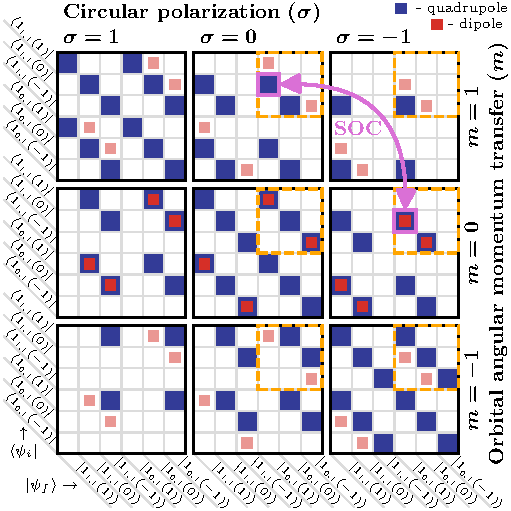
\includegraphics[width=\linewidth]{Figure1.pdf}
    \caption{非对称陀螺哈密顿量本征态之间允许的偶极跃迁(红色方框)与四极跃迁(蓝色方框)。各子图列表示光束的不同圆偏振态,子图行表示光束可传递给分子内转动的轨道角动量数值。紫色圆圈展示了自旋-轨道耦合产生携带轨道角动量转移的\eoet 项的示例。橙色方框标明了实验中会叠加的跃迁过程,如图\ref{fig:profiles}所示。}
    \label{fig:gridJ1}
\end{figure}
图~\ref{fig:gridJ1}的三列对应不同光束偏振,三行对应不同轨道角动量转移量子数$m$。如文献\cite{Maslov2024,Maslov_Thesis}所示,电偶极跃迁不转移轨道角动量,故仅出现在$m=0$行(但为便于比较,我们在$m=\pm 1$行也予以标注)。相反,电四极跃迁可转移最多一个轨道角动量量子($m=0,\pm 1$)。任何非平面波束通常包含所有三行的贡献,但其相对权重取决于具体的光场结构。

我们首先关注红蓝双色方框标记的态对——这些态间同时存在偶极和四极跃迁。它们全部出现在$m=0$行,表明跃迁过程无轨道角动量转移。这验证了表~\ref{SelectionRules}的结论,说明对于具有确定$\sigma$的光束,\eoet项无法产生HD,仅是对圆二色性(CD)的额外贡献。

然而,轨道角动量($m$)与自旋($\sigma$)的明确分离仅适用于傍轴光束。实际上,任何类型的光自旋-轨道耦合(SOC)都会导致不同$\sigma$分量的混合\cite{Bliokh2015,Bliokh2023}。这意味着图~\ref{fig:gridJ1}中不同面板的项可共同驱动同一跃迁。例如,紫色方框对应的\eoet项将同时涉及偶极跃迁($m=0$,$\sigma=-1$)和四极跃迁($m=0$,$\sigma=-1$与$m=1$,$\sigma=0$):$| 1_{0,1}(1) \rangle \to | 1_{1,1}(0) \rangle$。偶极矩项与$m=-1$四极分量的耦合使分子能够感知轨道角动量的影响。

实现此类跃迁所需的光自旋-轨道耦合可通过紧聚焦的拉盖尔-高斯光束产生\cite{Loeffler2011,Forbes2021nonparaxial,Forbes2021longitudinal}。我们采用一阶非傍轴近似描述光束\cite{Lax1975}(详见\cite{Note1}),并利用文献\cite{Maslov2024,Maslov_Thesis}的相互作用哈密顿量计算图~\ref{fig:gridJ1}虚线方框标记态间的空间分辨矩阵元。参数设置为:四极跃迁矩$Q_{xy}=0.5d_z\lambda$($d_z$为偶极跃迁矩,$\lambda$为波长),焦斑束腰$\omega_0=0.2\lambda$,离焦距离$z=\lambda$($z$为传播方向),拉盖尔-高斯光束的方位角拓扑荷$L_{\rm beam}=1$,偏振$\sigma=-1$。对映异构体通过分子固定(惯性)$xy$平面的反射描述。已有研究明确表明\cite{Buckingham1971, Power1975},观测\eoet相互作用需要各向异性,因此任何HD实验都必须分辨$M$态。图~\ref{fig:profiles}展示了$M$态分辨后的信号分布。

\begin{figure}[t!]
    \centering
    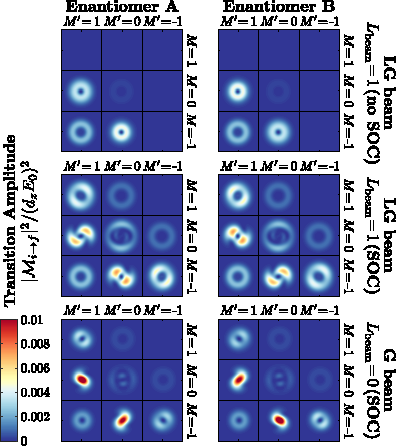
\includegraphics[width=1.0\columnwidth]{Figure2.pdf}
    \caption{对映异构体在拉盖尔-高斯光束耦合下(上)、自旋轨道耦合存在时(中)以及高斯光束与自旋轨道耦合共同作用时(下),从$\bra{1_{1,1}(M)}$态到$\ket{1_{0,1}(M')}$态的\eoet 跃迁信号剖面。}
    \label{fig:profiles}
\end{figure}
我们首先注意到,除非$d_zQ_{xy}^*$存在虚部${\rm Im}[d_zQ_{xy}^*]$,否则所有信号轮廓的积分值相等。虚部的存在会导致总吸收水平的二色性,这是已知的振动CD来源,其仅取决于分子内部参数而与电场结构无关(见\cite{Buckingham1971})。由此得出结论:仅通过光吸收强度无法检测HD,必须借助吸收剖面的空间分辨\cite{Loeffler2011}。

若无光自旋-轨道耦合,两个对映体间的唯一差异是$M=0\to M'=1$与$M=-1\to M'=0$剖面的强度(图~\ref{fig:profiles}顶行)。该二色性源于光束的$m=0$分量——即图~\ref{fig:gridJ1}中$\sigma=-1$、$m=0$面板虚线框内的红蓝方框。因此这是另一种空间分辨振动CD的来源,因其不涉及轨道角动量转移。

聚焦场引入的光自旋-轨道耦合导致了吸收剖面中新的对映体区分效应(图~\ref{fig:profiles}中行)。首先,$M=-1\to M'=0$与$M=0\to M'=1$跃迁的吸收存在显著差异。该信号源自图~\ref{fig:gridJ1}虚线方框中偶极与四极跃迁的耦合。这种差异源于涡旋光束与手性分子的相对螺旋性,并涉及轨道角动量转移,因此可视为真正的HD。
接下来,$M=1\to M'=1$与$M=-1\to M'=-1$的轮廓也存在差异。这源于虚线框中$\sigma=0$的偶极跃迁(图~\ref{fig:gridJ1})与$m=-1$、$\sigma=-1$方框中四极跃迁的耦合作用。因此,这也属于螺旋二色性(HD)。总体而言,自旋轨道耦合(SOC)光作用下的二色性信号强度比无耦合情况高出一个数量级。

图\ref{fig:profiles}最下行表明,在SOC情形下,渐近极限中无需使用携带轨道角动量(OAM)的光束。事实上,紧聚焦高斯光束同样能观测到HD现象。这是因为焦场会形成方位角电荷为$\sigma$的拉盖尔-高斯(LG)模式。实际上,紧聚焦线偏振光束也会呈现类似二色性,因其内部两个圆偏振分量通过SOC产生耦合。这说明入射光束的OAM与自旋均非观测HD的必要条件,关键在于光的自旋轨道耦合。

需注意,由于光SOC的作用,传递给分子的角动量类型难以明确区分,这阻碍了将所得二色性定性为圆二色性(CD)或螺旋二色性(HD)。我们的工作通过量子数$m$和$\sigma$(见图~\ref{fig:profiles})明确了OAM与自旋吸收通道,为解决该问题提供了途径。

总之,我们证明了傍轴OAM光束无法产生HD——这些条件下观测到的二色性均可归结为标准CD。真正的HD(与OAM转移直接关联的二色性)需要光的自旋-轨道耦合,如紧聚焦光束所示。引人注目的是,纯高斯模式在充分聚焦后也能展现真正的HD,尽管其在远场不携带OAM。这些发现阐明了结构光实验中HD的起源,并提示先前HD测量结果可能需要仔细复核以确认OAM转移的存在。特别是,未观测到二色性的研究要么主要探测偶极级相互作用\cite{Araoka2005},要么因信号平均化导致二色性丢失\cite{Loeffler2011};而成功检测到二色性的研究则同时利用了四极场相互作用和紧聚焦光束\cite{Rusak2019,Rouxel2022,Begin2023,Jain2023}。

本文建立的框架为设计基于光场空间结构的手性敏感光谱学及对映体分离方法提供了路线图~\cite{Leibscher2022}。\\
\begin{acknowledgments}
本研究全部或部分由奥地利科学基金(FWF)资助[项目编号:10.55776/F1004]。
\end{acknowledgments}
\bibliography{bibliography}
\end{document}
